\chapter{基于深度相机模型形变捕捉}
要构建模型的形变子空间,除了静态三维模型,
还需要一些形变后的模型,即形变关键帧作为输入。
本章描述了一个以静态模型和深度视频为输入的形变捕捉算法。
在捕捉步骤中,操作者会带着特定颜色的手套,在深度相机前摆弄物体,使得物体发生形变。
该算法会优化模型的形变参数,使得模型的形状和相机采集的物体形状尽量吻合,
从而得到形变后的模型。
本文会从捕捉到的形变中选取若干成为形变关键帧,作为形变子空间构建的输入。
本章接下来就会阐述该算法的技术细节。

\section{模型初始位姿估计}

 类似于三维重建步骤中的相机位姿估计,
 在形变步骤中,对于每一帧深度图像,本文仅计算模型和上一帧的相对形变。
 因此,在捕捉形变之前,需要得知模型的初始位置。
 在本文的形变捕捉流程中,操作者需要用手持物。
 所以物体必然位于手的附近,所以本文设计了一个借助手部信息确定模型的初始位置与朝向的算法。
 本位所采用的确定物体初始位姿的算法可主要分为三个步骤:分割手部点云、分割物体点云、模型对齐。
 本节接下来就会详细描述这一流程。

\subsection{手部点云分割}
由于本文是借助手部点云的位置寻找物体的点云,
所以需要在输入的点云中分割出属于手的部分。
本节就将描述一种基于RGBD图像的点云分割算法。
\begin{figure}[h]
    \centering
    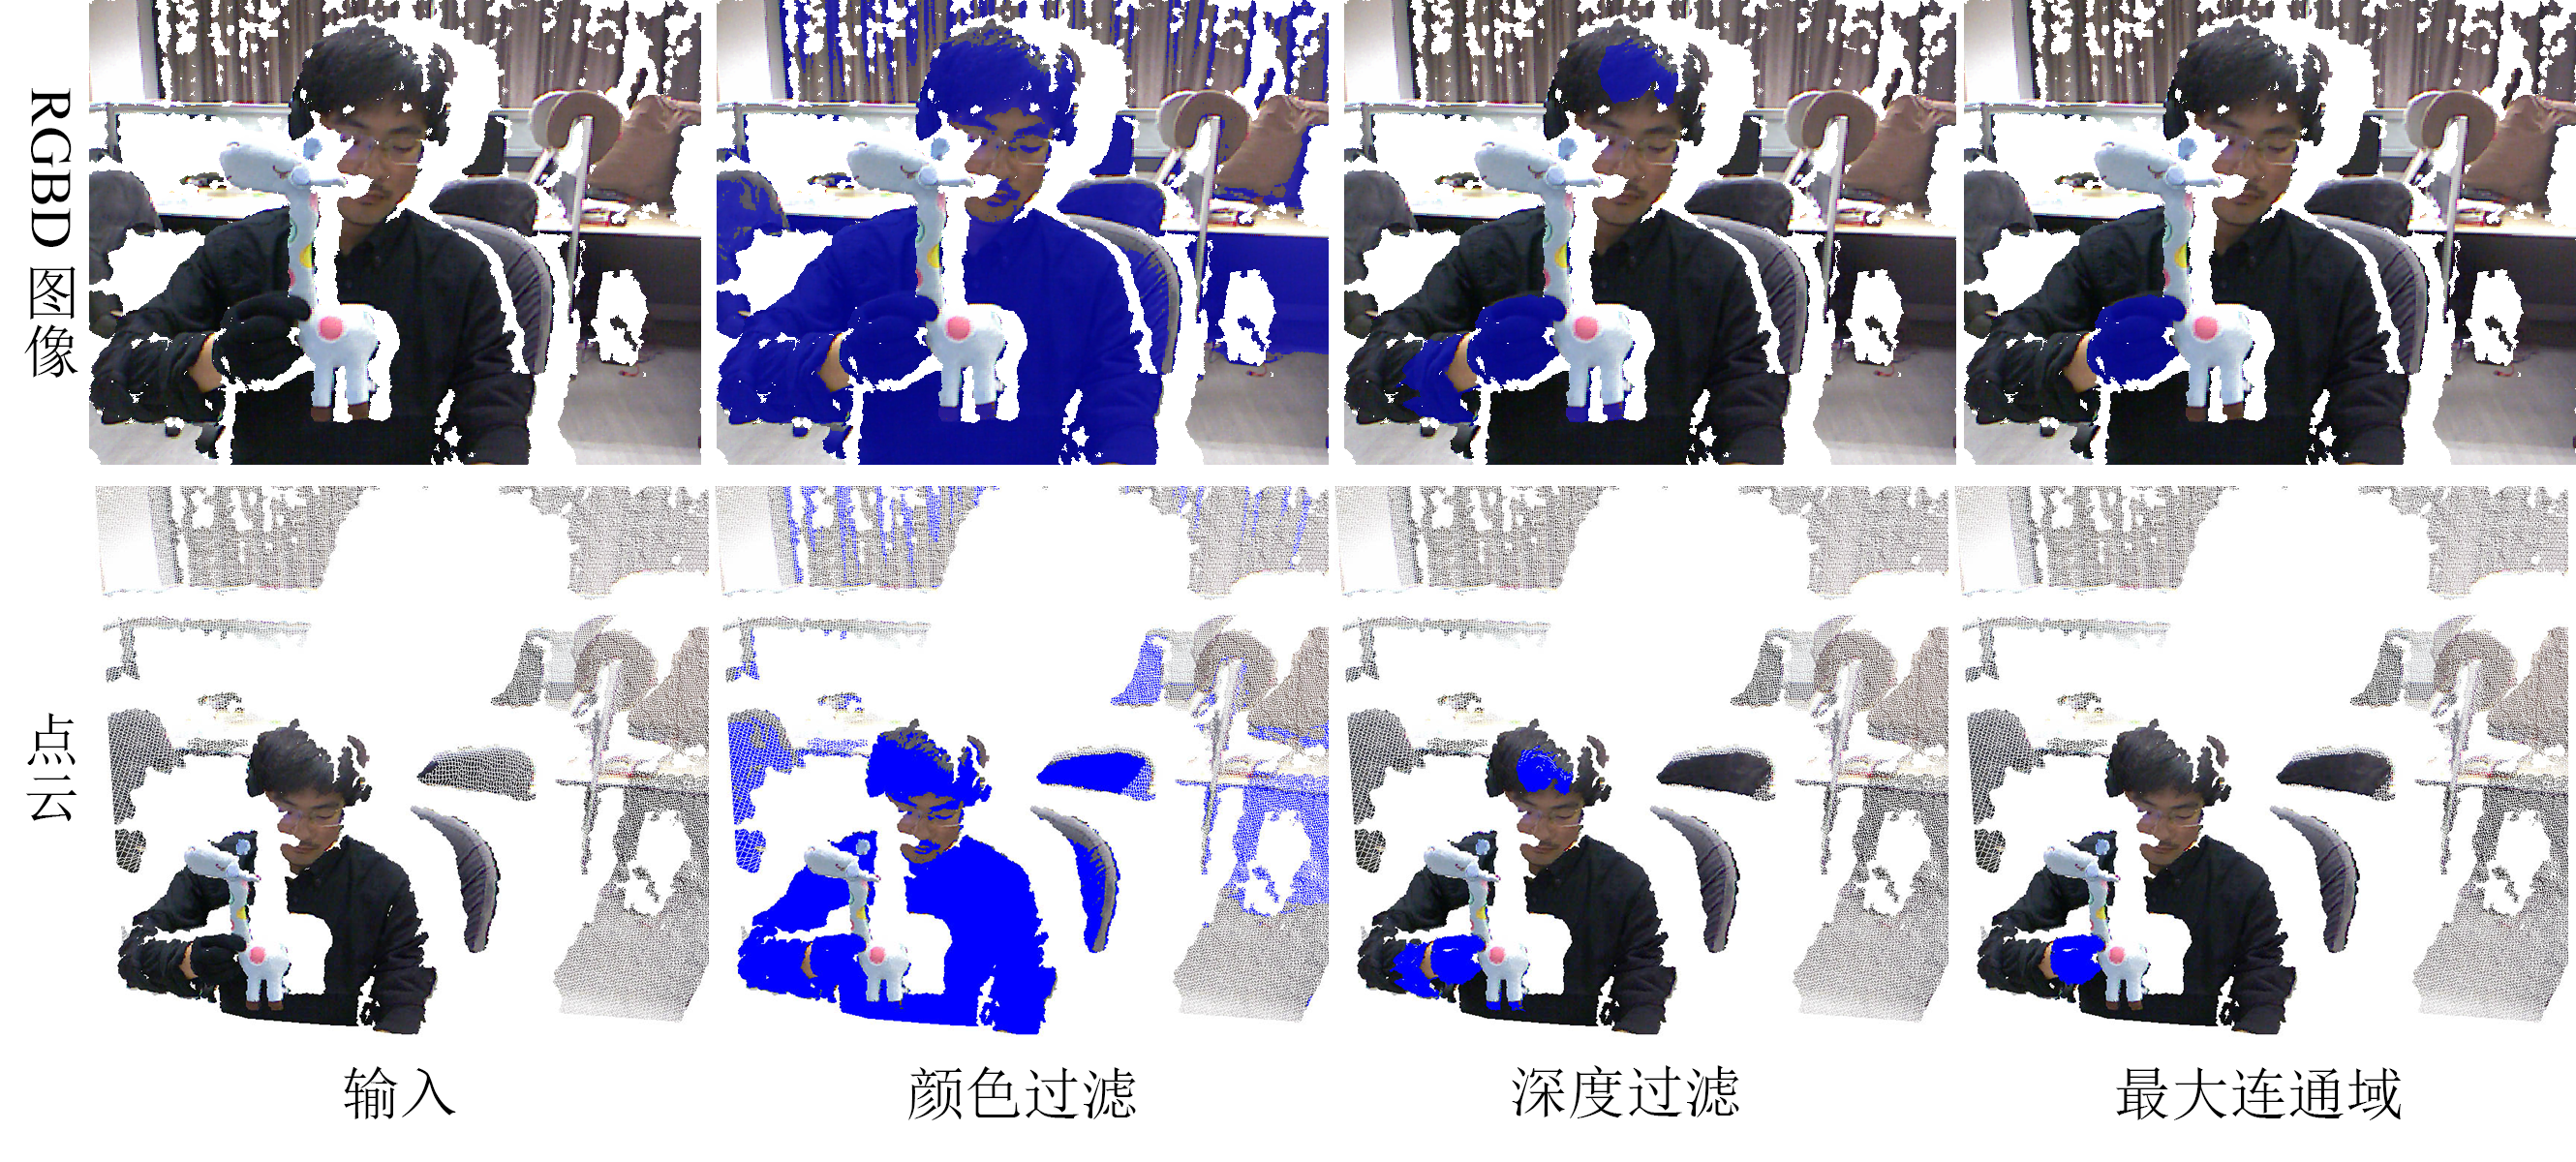
\includegraphics[width = \textwidth]{./Pictures/FindingHand.png}
    \caption{手部点云分割流程}
    \label{finding_hand}
\end{figure}
分割手部点云阶段的输入是RGBD图像,输出为手部的像素坐标的集合。
RGBD图像即除了RGB三个颜色通道外,还有一个深度通道
记录了对应点距离相机的距离,可以理解为RGB图像加上深度图像。
Kinect分别通过色彩传感器和深度传感器获得RGB图像和深度图像,
由于两个传感器的相对位置被事先标定过,
所以Kinect的SDK提供了将RGB图像映射到深度图像的接口,
映射后的RGB图像的像素和深度图像的像素一一对应。
图\ref{finding_hand}第一行的第一张图就是映射到相应深度图位置后的RGB图像。
本文中提到的RGB图像均默认指映射后的RGB图像。

在操作物体时,操作者会带上特定颜色的手套,以对相应的数据做特殊处理。
找出手部数据的主要目的是在后续的形变捕捉步骤中过滤掉所有手部的深度信息,
因为手部的深度信息对于形变捕捉是很大的噪声。
在形变捕捉的前置阶段——初始位置阶段,
手部信息也作为辅助信息用于确定物体的初始位姿
如图\ref{finding_hand}和算法\ref{alg_seg_hand}所示,
分割手部点云阶段可主要分为颜色过滤、深度过滤、寻找最大连通域三个步骤。
图\ref{finding_hand}的第一行的图片中被标记为蓝色的部分是每个步骤确定的手的位置,
第二行的图片是对应的点云。
\begin{algorithm}
    %\fangsong
    \caption{分割手部点云}
    \label{alg_seg_hand}
    \begin{algorithmic}[1]
        %\Require RGB图像$\bm{C_i}$,深度图像$\bm{D_i}$
        %\Ensure 手部像素集合$\bm{S_{hand}}$
        %\rm
        \Procedure{GetHandPixels}{$\bm{C_i}$, $\bm{D_i}$}
            %\State $\bm{V_i} \gets$ \Call{DepthToVertex}{$\bm{D_i}$}
            \State $\bm{S_{hand1}} \gets$ \Call{ColorFilter}{$\bm{C_i}$}
            \State $\bm{S_{hand2}} \gets$ \Call{DepthFilter}{$\bm{D_i}$, $\bm{S_{hand1}}$, $thd_{hand}$}
            \State $\bm{S_{hand3}} \gets$ \Call{LargestConnectedDomain}{$\bm{S_{hand2}}$}
        \EndProcedure
    \end{algorithmic}
\end{algorithm}
% \begin{algorithm}
%     \fangsong
%     \caption{分割手部点云}
%     \label{alg_seg_hand}
%     \begin{algorithmic}[1]
%         \Require RGB图像$\bm{C_i}$,深度图像$\bm{D_i}$
%         \Ensure 手部像素集合$\bm{S_{hand}}$
%         \Procedure{GetHandPixels}{$\bm{C_i}$, $\bm{D_i}$}
%             %\State $\bm{V_i} \gets$ \Call{DepthToVertex}{$\bm{D_i}$}
%             \State $\bm{S_{hand}} \gets$ 
%                    $\{$
%                    $\bm{u} \in$ \Call{PixelDomain}{\bm{D_i}}
%                    $|$
%                    $\nexists \bm{c} \in \bm{C_{hand}} :$
%                    $\| \bm{C_i}(\bm{u}) - \bm{c}\| \leq thd_{color}$
%                    $\}$
%             \State $\bm{S_{hand}} \gets$ \Call{DepthFilter}{$\bm{D_i}$, $\bm{S_{hand}}$}
%             \State $\bm{S_{hand}} \gets$ \Call{LargestConnectedDomain}{$\bm{S_{hand}}$}
%         \EndProcedure
%     \end{algorithmic}
% \end{algorithm}

首先,本文会进行颜色过滤步骤,筛选出输入图像中与手套颜色相近的像素点。
算法\ref{alg_cfilter}描述了颜色过滤的流程。
其中$\bm{C_{hand}}$和$thd_{color}$分别是预先设定的手套颜色的集合和颜色距离阈值。
本文的实验中$thd_{color}$的值设为50。
在该步骤中,会遍历RGB图像的每一个像素。
如果该像素的颜色和$\bm{C_{hand}}$中的任何颜色相近,
即在RGB颜色空间中与相应颜色距离小于$thd_{color}$的像素,
就会被认为可能是手部的像素,并入待选集合中。
遍历结束后,就会得到符合颜色要求的候选集合。
\begin{equation}
    \bm{S_{hand1}} \gets
    \{
    \bm{u} \quad
    | \quad
    \exists \bm{c} \in \bm{C_{hand}} :
    \| \bm{C_i}(\bm{u}) - \bm{c}\| \leq thd_{color}
    \}
\end{equation}
颜色过滤的记过如图\ref{finding_hand}中第二列所示。
从图中可以看出,颜色过滤会将图像背景中大量颜色与手套相近的像素判定为手部像素。
所以,如果要借助手的位置确定物体的位置,还需要进一步的筛除背景中多余的像素。
\begin{algorithm}
    %\fangsong
    \caption{颜色过滤}
    \label{alg_cfilter}
    \begin{algorithmic}[1]
        %\Require RGB图像$\bm{C_i}$
        %\Ensure 像素点集合$\bm{S}$
        %\rm
        \Function {ColorFilter}{$\bm{C_i}$}
            % \State $\bm{S_out} \gets \varnothing$
            \For {$\forall\bm{u} \in$ \Call{PixelDomain}{$\bm{C_i}$}}
                \For {$\forall\bm{c} \in \bm{C_{hand}}$}
                    \If{$\|\bm{C_i}(u) - \bm{c}\| \leq thd_{color}$}
                    \State $\bm{S_{out}} \gets \bm{S_{out}} \bigcup \{\bm{c}\}$
                    \EndIf
                \EndFor
            \EndFor 
            % \State $\bm{S} \gets$ 
            %        $\{$
            %        $\bm{u} \in$ \Call{PixelDomain}{$\bm{C_i}$}
            %        $|$
            %        $\exists \bm{c} \in \bm{C_{hand}} :\quad$
            %        $\| \bm{C_i}(\bm{u}) - \bm{c}\| \leq thd_{color}$
            %        $\}$
            \State \Return $\bm{S_out}$
        \EndFunction
    \end{algorithmic}
\end{algorithm}

在颜色过滤后,本文会执行深度过滤步骤,即只保留深度最小像素点。
从图\ref{finding_hand}中可以看出,在操作者手持物体操作的过程中,
握着物体的手总是位于最前方。
%在这种特定的场景中,本文默认手部的像素点必在深度值最小的那部分像素之中。
算法\ref{alg_dfilter}描述了深度过滤的流程。
其中,$d_{range}$是预先设定的筛选深度范围,%在本文的实验中设为150毫米。
$d_{min}$是集合中深度最小的像素的深度值。
然后遍历集合中的每个像素,仅保留深度值小于$d_{min}+d_{range}$的像素。
\begin{equation}
    \bm{S_{hand2}} \gets
    \{
    \bm{u} \in \bm{S_{hand1}} \quad
    | \quad
    d_{dim} \leq \bm{D_i}(\bm{u}) \leq d_{min} + d_{range}
    \}
\end{equation}
深度过滤的结果如图\ref{finding_hand}第三列所示。
% \begin{algorithm}
%     \fangsong
%     \caption{深度图像转点云}
%     \label{alg_d2v}
%     \begin{algorithmic}
%         \Require 深度图像$\bm{D_i}$
%         \Ensure 点云$\bm{V_i}$
%         \Function {DepthToVertex}{$D_i$}
%             \For{$\forall \bm{u} \in$ \Call{PixelDomain}{$\bm{D_i}$}}
%                 \State $\bm{V_i(u)}=\bm{D_i}(\bm{u})\bm{K}^-1[\bm{u},1]$
%             \EndFor
%             \State \Return $\bm{V_i}$
%         \EndFunction
%     \end{algorithmic}
% \end{algorithm}
\begin{algorithm}
    %\fangsong
    \caption{深度过滤}
    \label{alg_dfilter}
    \begin{algorithmic}[1]
        %\Require 深度图像$\bm{D_i}$, 像素点集合$\bm{S_{in}}$,深度阈值$d_{range}$
        %\Ensure 像素点集合$\bm{S_{out}}$
        %\rm
        \Function {DepthFilter}{$\bm{D_i}$, $\bm{S_{in}}$, $d_{range}$}
            % \State $\bm{Set_{out}} \gets \varnothing$
            \State $d_{min} \gets$ \Call{Min}{$\bm{D_i}$}
            \For {$\forall \bm{u} \in \bm{S_{in}}$}
                \If {$d_{dim} \leq \bm{D_i}(\bm{u}) \leq d_{min} + d_{range}$}
                    %\State $\bm{Set_out} \gets \bm{S} - \{u\}$
                    \State $\bm{S_{out}} \gets \bm{S_{out}} \bigcup \{\bm{u}\}$
                \EndIf
            \EndFor
            % \State $\bm{S_{out}} \gets$ 
            %        $\{$
            %        $\bm{u} \in \bm{S_{in}}$
            %        $|$
            %        $d_{dim} \leq \bm{D_i}(\bm{u}) \leq d_{min} + d_{range}$
            %        $\}$
            \State \Return $\bm{S_{out}}$
        \EndFunction
    \end{algorithmic}
\end{algorithm}
\begin{algorithm}
    %\fangsong
    \caption{获取最大连通域}
    \label{alg_lcd}
    \begin{algorithmic}[1]
        %\Require 像素点集合$\bm{S}$
        %\Ensure 最大连通域$\bm{LCD}$
        \rm
        \Function {LargestConnectedDomain}{$\bm{S}$}
            % \State $\bm{LCD} \gets \varnothing$
            \For{$\forall \bm{u} \in \bm{S}$}
                \If{$\bm{u}$ not checked}
                    \State $\bm{CD} \gets$ \Call{GetConnectedDomain}{$\bm{S}$, $\bm{u}$}
                    \If{$|\bm{CD}| > |\bm{LCD}|$}
                        \State $\bm{LCD} \gets  \bm{CD}$
                    \EndIf
                \EndIf
            \EndFor
            \State \Return $\bm{LCD}$
        \EndFunction
        \Function {GetConnectedDomain}{$\bm{S}$, $\bm{u}$}
            % \State $Q \gets$ \Call{EmptyQueue}{}
            % \State $\bm{CD} \gets \varnothing$
            \State \Call{QueuePush}{$Q$, $\bm{u}$}
            \State set $\bm{u}$ as checked
            \While{$Q$ not empty}
                \State $\bm{u_i} \gets$ \Call{QueuePop}{$Q$}
                \State $\bm{CD} \gets \bm{CD} \bigcup \{\bm{u_i}\}$
                \For{$\forall \bm{u_{neighbor}} \in$ \Call{NeighborPixel}{$\bm{u_i}$}}
                    \If{$\bm{u_{neighbor}}$ not checked and $\bm{u_{neighbor}} \in \bm{S}$}
                        \State \Call{QueuePush}{$Q$, $\bm{u_{neighbor}}$}
                        \State set $\bm{u_{neighbor}}$ as checked
                    \EndIf
                \EndFor
            \EndWhile
            \State \Return $\bm{CD}$
        \EndFunction
    \end{algorithmic}
\end{algorithm}
在深度过滤后,本文将在已经判定为手部的像素集合中找到其在图像空间中最大连通域,
进一步去除零散的像素点。
以带黑色手套为例,这些被误判的像素点可能是物体上阴影所在的部分,
也可能是身体靠近物体的部分。
这些被误判的区域会影响物体位置的估计。
在实验的过程中可以发现,在深度过滤之后,真正的手部在图像中,
大都落在已判定区域中的最大连通域里。
所以本文在深度过滤的结果中寻找图像空间中的最大连通域,作为最终的手部区域。
算法\ref{alg_lcd}描述了该步骤的流程。
GetConnectedDomain函数采用了广度优先搜索的方式计算与指定像素位置$\bm{u}$
相连的连通域。
每个像素被看做与上下左右四个相邻像素相连。
在整个计算最大连通域的过程中,程序会维护一张全局的状态表,记录每个像素是否被访问过。
在遍历时,每一个被访问的像素都会被标记为已访问。
LargestConnectedDomain函数遍历了集合中所有的连通域,并从中找出最大的连通域。
它会遍历候选集合中的每一个像素,若该像素还未被访问过,则调用GetConnectedDomain函数计算其连通域,
若该连通域比之前访问过的连通域都大,则将该连通域记录为最大连通域。
在遍历完成后,就能得到候选集合在图像空间中的最大连通域。
最终分割出的手部点云如图\ref{finding_hand}第四列所示。

在上述步骤中,颜色过滤和深度过滤各像素位置的计算是互相独立的,可用GPU并行加速。
其中颜色过滤在实现时与RGB图映射到深度图的步骤在同一个CUDA Kernel中实现。
最大连通域的计算需要根据各像素的邻接关系,不便于大规模并行。
且经由之前的筛选,该步骤需要遍历的像素已大为减少,所以在CPU上可以很快的完成。


\subsection{物体点云分割}
在后续的模型对齐操作中,
且输入中那些不属于物体的点云,会影响物体位置的估计且容易造成对齐过程中的误匹配。
所以,为了提高模型匹配的效果,本文需要将模型的点云从数据中分割出来。
如前文所说,由于在采集数据的过程中,操作者会手持物体,
所以物体必定位于手的附近。
下文就将描述一种借助手部信息,在根据深度图像生成的点云中分割物体点云的算法。
如图\ref{finding_object}和算法\ref{alg_seg_obj}所示,
物体点云分割主要分为半径过滤、深度过滤、寻找最大连通域三个步骤。
\begin{figure}[ht]
    \centering
    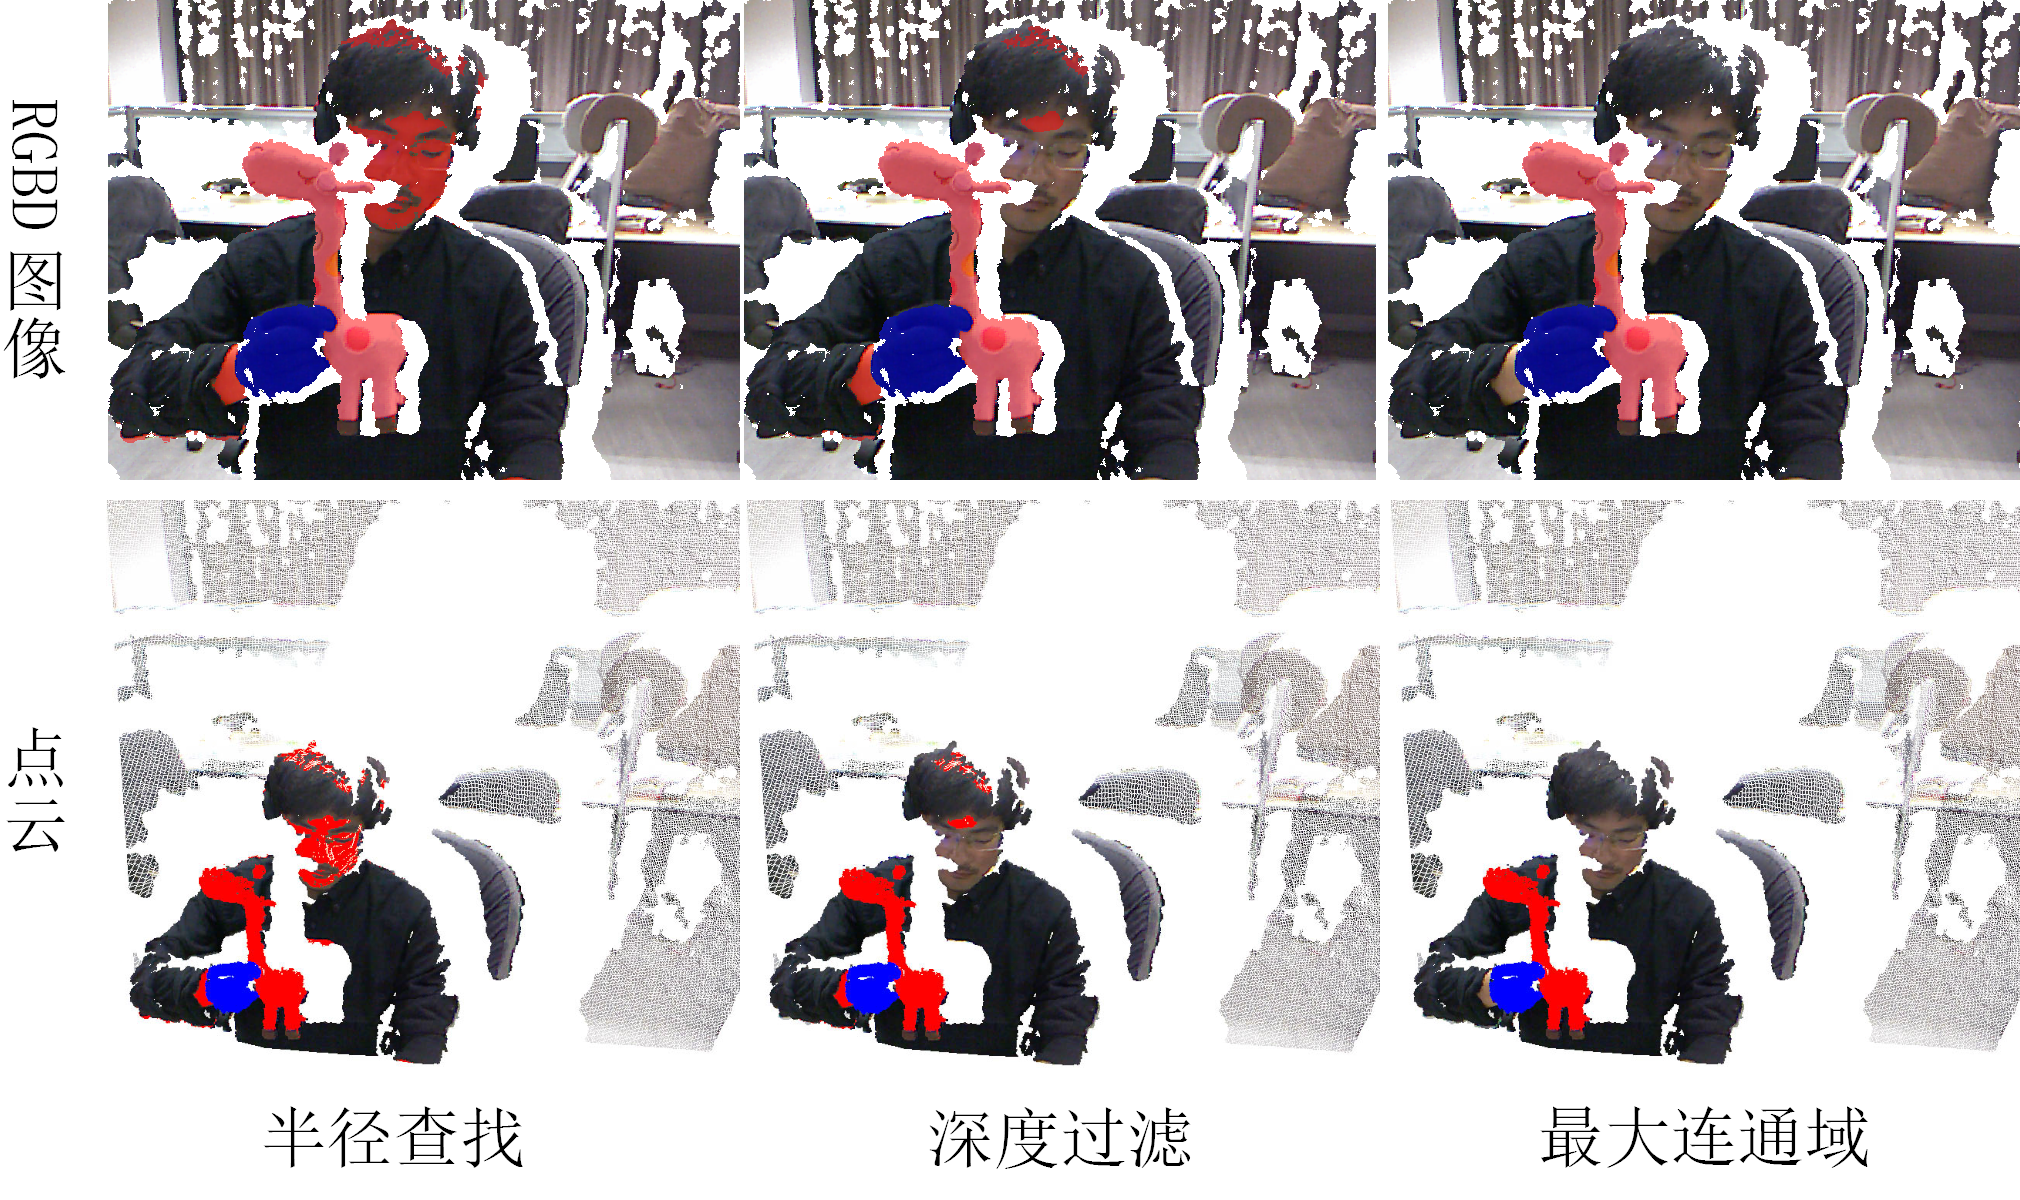
\includegraphics[width = 0.75\textwidth]{./Pictures/FindingObj.png}
    \caption{物体点云分割流程}
    \label{finding_object}
\end{figure}
\begin{algorithm}
    %\fangsong
    \caption{物体点云分割}
    \label{alg_seg_obj}
    \begin{algorithmic}[1]
        %\Require 深度图像$\bm{D_i}$, 手部像素点集合$\bm{S_{hand}}$, 网格模型$\bm{m_{object}}$
        %\Ensure 物体像素点集合$\bm{S_{object}}$
        %\rm
        \Procedure{GetObjectPixels}{$\bm{D_i}$, $\bm{S_{hand}}$,$\bm{m_{object}}$}
            \State $d \gets$ the diagonal length of the bounding box of mesh $\bm{m_{object}}$
            \State $size_z \gets$ the size of the bounding box of mesh $\bm{m_{object}}$ in $z$ dimension
            \State $\bm{S_{object1}} \gets$ \Call{RadiusFilter}{$\bm{D_i}$, ${\lambda}_{r}\frac{d}{2}$, $\bm{S_{hand3}}$}
            \State $\bm{S_{object2}} \gets$ \Call{DepthFilter}{$\bm{D_i}$, $\bm{S_{object1}}$,${\lambda}_d size_z$}
            \State $\bm{S_{object3}} \gets$ \Call{LargestConnectedDomain}{$\bm{S_{object2}}$}
        \EndProcedure
    \end{algorithmic}
\end{algorithm} 

分割手部点云的第一步是半径过滤,即分割出空间中指定的球形区域内的点云。
\begin{equation}
    \bm{S_{object1}} =
    \{
        \bm{u} \quad
    |   \quad
        \|\bm{V_i}(\bm{u}) - \bm{center_{hand}}\| \leqslant {\lambda}_{r}\frac{d}{2}
        \quad and \quad
        \bm{u}\notin \bm{S_{hand3}}
    \}
\end{equation}
其中$d$为上一章中重建得到的网格模型$m_{object}$的包围盒的对角线长度,
${\lambda}_r$为根据经验人工指定的放大系数。
在本文的实验中${\lambda}_r=1.5$。
半径过滤会筛选出落在上述球形区域中且不属于手部的点云。
图\ref{finding_object}(左)中红色的部分即半径过滤所筛选出的物体点云。
\begin{algorithm}
    %\fangsong
    \caption{半径过滤}
    \label{alg_rfilter}
    \begin{algorithmic}[1]
        %\Require 深度图像$\bm{D_i}$, 手部像素点集合$\bm{S_{hand}}$, 网格模型$\bm{m_{object}}$
        %\Ensure 物体像素点集合$\bm{S_{object}}$
        \Function{RadiusFilter}{$\bm{D_i}$, $r$, $\bm{S_{hand3}}$}
            %\State $\bm{S_{out}} \gets \varnothing$
            \State $\bm{V_i} \gets$ \Call{DepthToVertex}{$\bm{D_i}$}
            \State $\bm{center_{hand}} \gets$ the center of the bounding box of point cloud $\bm{V_i}(\bm{S_{hand3}})$
            \For{$\forall \bm{u} \in$ \Call{PixelDomain}{$\bm{V_i}$}}
                \If{$ \|\bm{V_i}(\bm{u}) - \bm{center_{hand}}\| \leqslant r$ and $\bm{u}\notin \bm{S_{hand3}}$}
                    \State $\bm{S_{out}} \gets \bm{S_{out}} \bigcup \{u\}$
                \EndIf
            \EndFor
            % \State $\bm{S_{object}} \gets$
            %        $\{\bm{u} \in$ \Call{PixelDomain}{$\bm{V_i}$}
            %        $|$
            %        $ \|\bm{V_i}(\bm{u}) - \bm{center_{hand}}\| \leqslant r$
            %        $\quad and \quad$
            %        $ \bm{u}\notin \bm{S_{hand}}$
            %        $\}$
            \State \Return $\bm{S_{out}}$
        \EndFunction
    \end{algorithmic}
\end{algorithm} 

出于同样的理由,与手部点云分割一样,
经由半径过滤筛选出的点云也会经由深度过滤和寻找最大连通域进行进一步筛选:
深度过滤筛选出位于最前方的那部分候选点云,最大连通域会剔除那些零散的手附近的点云。
在分割物体点云的步骤中,
深度过滤的阈值$d_{range} = {\lambda}_{d} size_z$同样可以根据网格模型$m_{object}$的包围盒估计。
其中$size_z$为包围盒在$z$方向上的长度,${\lambda}_d$为根据经验人工指定的放大系数。
本文的实验中${\lambda}_d = 1.2$。
图\ref{finding_object}(中)(右)中红色的部分分别为深度过滤和寻找最大连通域所筛选出的点云。
可以看出经过一些列的筛选,本文可以很好的从输入的点云中分割出物体的点云。
\subsection{模型对齐}

经由前两节的筛选,本文分割出了物体的点云,如图\ref{rigid_fit}(左)所示。
根据点云的包围盒的中心位置,可以得到物体的大致位置。
但物体的朝向还需要让分割出的点云和上一章重建得到的网格模型对齐后才能确定。
图\ref{rigid_fit}(中)即为将模型平移至点云中心后的结果,
可以看出,还需要进行进一步模型的位姿优化才能使模型与点云对齐,
得到一个较为准确的初始位姿。

点云对齐是一个由来已久的问题:给定源点云$\bm{P}$和目标点云$\bm{Q}$,
需要计算一个最优的刚体变换$\bm{T}$,使得$\bm{TP} \approx \bm{Q}$。
ICP是最为常见的用于点云对齐的算法。
但ICP算法是一个局部的刚体变换估计算法,它需要一个十分靠近最优位置的初始值,
即源点云和目标点云之间只能存在微小的偏移。
所以ICP只能用来估计微小的、局部的刚体变换,
并不适用于本文在当前步骤所需要解决的问题。
本文采用Super 4PCS算法\cite{mellado2014super}进行模型与点云的对齐。
Super 4PCS是改良后的4PCS算法(4-Points Congruent Sets)\cite{aiger20084},
是一种高效的全局点云对齐算法。
\begin{figure}
    \centering
    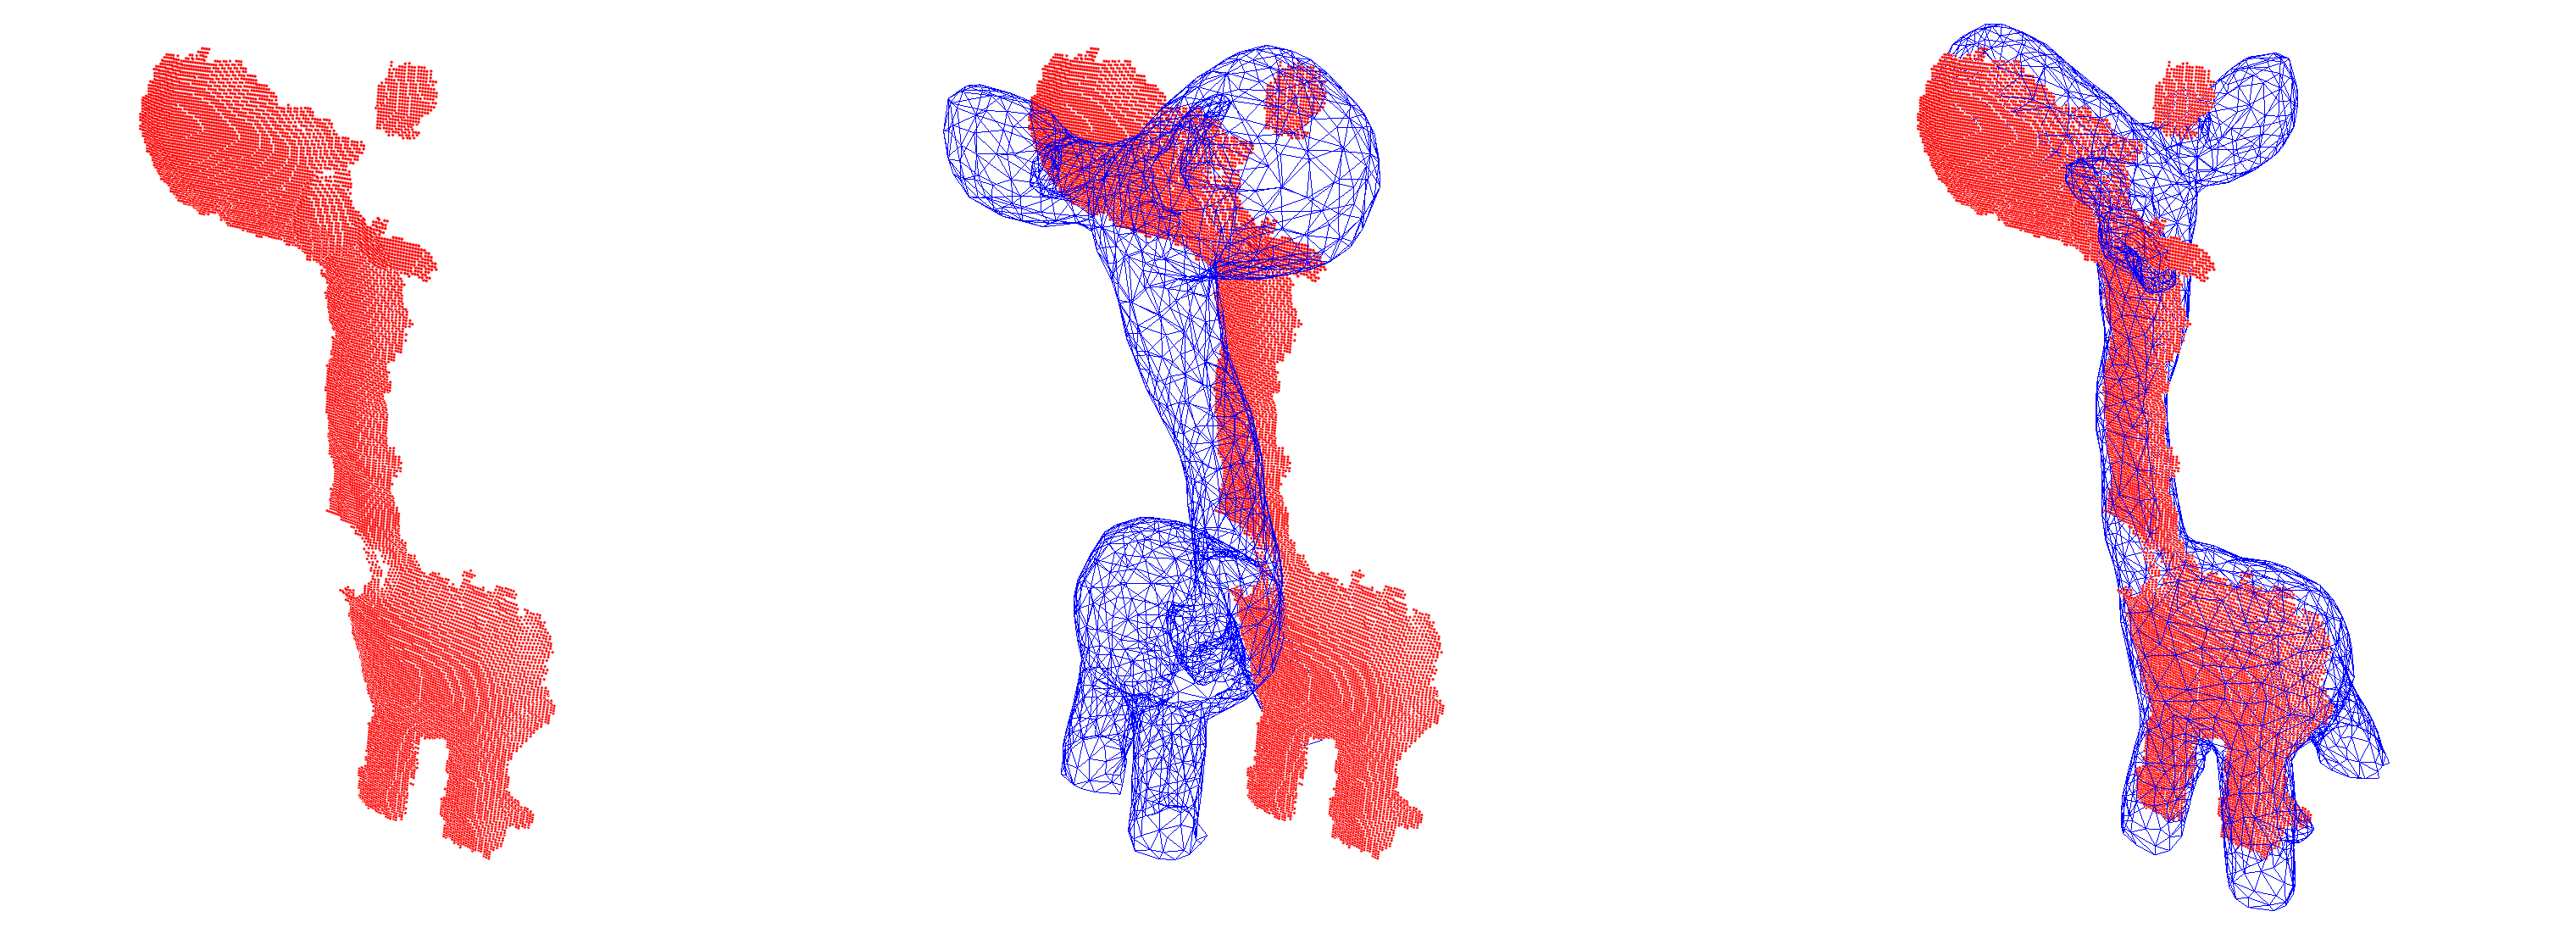
\includegraphics[width = \textwidth]{./Pictures/rigidfitting.png}
    \caption{模型与点云对齐}
    \label{rigid_fit}
\end{figure}

4PCS是四点全等集的缩写,其核心思想是通过计算小的共面点集的空间变换来代替大点云的空间变换。
众所周知,三维空间中三个及三个以上不共线的点就能够定义出三维空间中的位置与朝向。
4PCS算法用点云中共面(不共线)四个点描述点云的空间变换。
4PCS算法每次计算时在源点云$\bm{P}$
中选取共面的四个点作为基点集$\bm{B}=\{\bm{a},\bm{b},\bm{c},\bm{d}\}$,
然后找出目标点云$Q$中所有与$\bm{B}$全等的四点集
$\bm{CS}=\{\bm{q_1},\bm{q_2},\bm{q_3},\bm{q_4}\}$,
计算$\bm{B}$到$\bm{CS}$的刚体变换。
在遍历了所有的全等四点集后,选择其中最优的变换作为点云$\bm{P}$到$\bm{Q}$的变换。
借助全等(相似)变换的性质,可以利用高效的空间数据结构快速的找出全等点集。
4PCS算法就利用了全等变换后线段比例不变的性质和range tree数据结构进行全等点集的查找。
不过由于4PCS仅仅根据线段比例判定点集是否相似,并不考虑线段间的夹角不变,
会将一些并与基点集$\bm{B}$相似的点集也记录下来。
更具体的细节可以查阅4PCS的论文做进一步的了解。
4PCS算法的时间复杂度为$O(n^2+k)$,$n$为点云$\bm{Q}$中顶点的数目,
$k$为$\bm{Q}$中找到全等点集的数目。
在算法中查找所有全等点集的时间复杂度为$O(n^2)$,
在$k$点集的对应的变换中找出最优变换的时间复杂度为$O(k)$。

Super 4PCS算法主要在4PCS的时间复杂度上做了进一步的优化。
首先,它采用了栅格化的数据结构将查找全等点集的时间复杂度优化到$O(n)$;
此外,Super 4PCS算法在判定相似关系时还考虑了对角线的夹角,除去了4PCS中冗余的点集,降低了$k$的值。
所以,Super 4PCS算法的时间复杂度为$O(n+k)$,并拥比原始的4PCS有更小的$k$值。
\begin{figure}
    \centering
    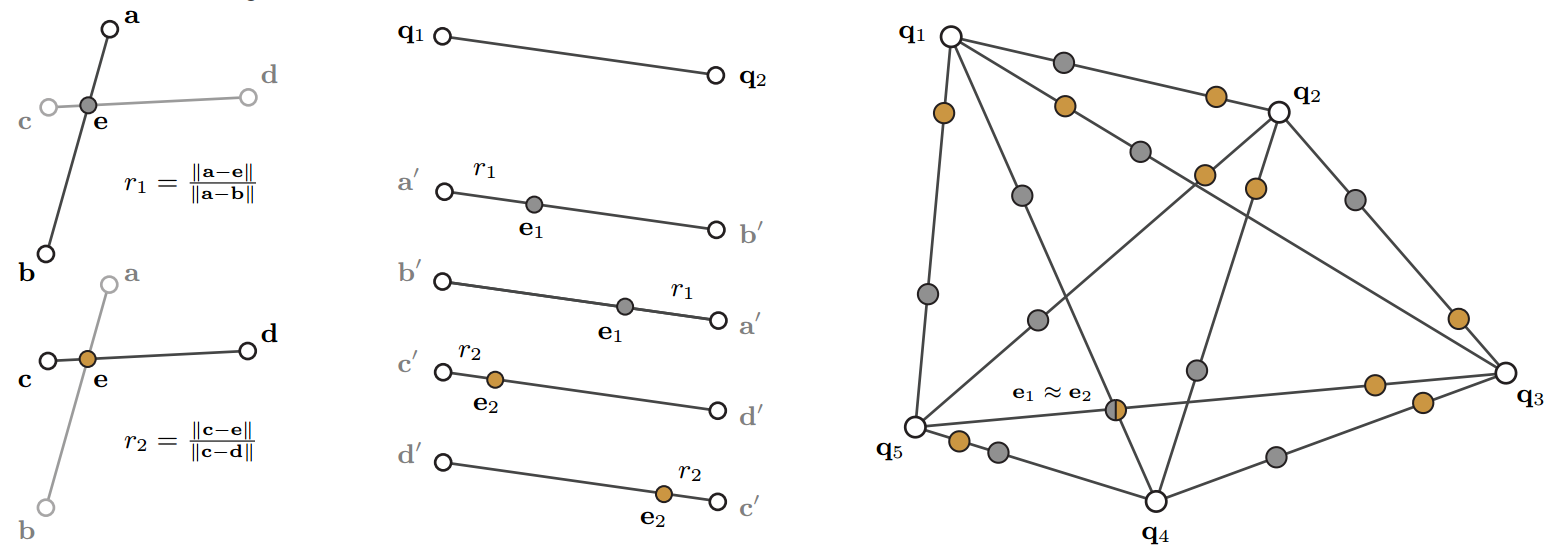
\includegraphics[width = \textwidth]{./Pictures/4PCS.png}
    \caption{4PCS算法利用对角线交点的分割比判定相似关系}
    \label{4pcs}
\end{figure}

在本文的应用场景中,需要估计网格模型$\bm{m_{object}}$到点云
$\bm{Q_{object}} = \bm{V_i}(\bm{S_{object}})$的刚体变换$\bm{T_{m2o}}$。
但由于深度图像仅仅采集了物体朝向相机那一侧的深度信息,
点云$\bm{Q_{object}}$只包含了部分的物体表面,
而网格模型$\bm{m_{object}}$包含了完整的物体表面信息。
所在,如果以$\bm{m_{object}}$为源点云,
在$\bm{m_{object}}$中选取的基点集$\bm{B}$中可能会有未被点云$\bm{Q_{object}}$包含的区域。
所以,本文在使用Super 4PCS算法估计刚体变换时,以点云$\bm{Q_{object}}$为源,
以网格模型$\bm{m_{object}}$为目标,得到变换矩阵$\bm{T_{o2m}}$,
然后对其求逆得到变换矩阵${T_{m2o}=\bm{T_{o2m}}}^{-1}$。
图\ref{rigid_fit}(右)即为模型与点云对齐后的结果。

\section{形变捕捉}
\subsection{形变的参数化描述}
\subsection{形变参数优化}

\section{本章小结}